\documentclass{ucbthesis}

% Double spacing, if you want it.
% \def\dsp{\def\baselinestretch{2.0}\large\normalsize}
% \dsp

% If the Grad. Division insists that the first paragraph of a section
% be indented (like the others), then include this line:
% \usepackage{indentfirst}


% For revision control
\usepackage{rcs-multi}
\rcsid{$Id$}
\rcsid{$Header$}
\rcskwsave{$Author$}
\rcskwsave{$Date$} 
\rcskwsave{$Revision$}
%\rcsRegisterAuthor{devangel}{Dennis Jos{\'e} Evangelista}
\rcsRegisterAuthor{devangel}{Dennis J. Evangelista}

% I typically use these
\usepackage{graphicx}
\usepackage[usenames,dvipsnames]{color}
\usepackage{makeidx}
\usepackage{siunitx}
\usepackage{rotating}

% PDF metadata
\usepackage{url}
\usepackage{hyperref}
\hypersetup{pdftitle={Something about Aerial Righting, Directed Aerial Descent, Maneuverability and Stability, and their Implications for the Evolution of Flight in Vertebrates}}
%\hypersetup{pdfauthor={Dennis Jos{\'e} Evangelista}}
\hypersetup{pdfauthor={Dennis J. Evangelista}}
\hypersetup{pdfsubject={biomechanics}}
\hypersetup{pdfkeywords={biomechanics, evolution, integrative biology, organismic}}
\hypersetup{colorlinks=true,citecolor=Violet,linkcolor=Blue,urlcolor=Red}
\hypersetup{bookmarks=true,bookmarksopen=true,hyperfootnotes=false,pdfpagemode=UseOutlines}

% Biology style references
\usepackage[round, sort&compress]{natbib}
\setcitestyle{authoryear, round, comma, aysep={;}, yysep={,}, notesep={, }}
\bibliographystyle{abbrvnat}
%\def\newblock{\hskip .11em plus .33em minus .07em} % bug workaround
% show doi in citations
\newcommand*{\doi}[1]{\href{http://dx.doi.org/\detokenize{#1}}{\texttt{doi:\detokenize{#1}}}}
\renewcommand\bibname{References}
\usepackage{bibentry}


% For chapter bibliographies
%\usepackage[sectionbib,duplicate]{chapterbib}

% For chapter abstracts
%\newenvironment{chabstract}{\begin{quote}\small}{\end{quote}}
%\newenvironment{chabstract}{\section*{}}{}

% Set section depth on table of contents
\setcounter{secnumdepth}{3}

% Use AMS math
\usepackage{amsmath}

% Yonatan used these?
%\usepackage{setspace}
%\usepackage{lscape}
%\usepackage{lineno}   % line numbering
%\modulolinenumbers[5] % line numbering
%\usepackage[hang,small,bf]{caption} % captions?
%\usepackage{xspace}

% Commands for Genus species names
\newcommand{\species}[1]{\emph{#1}}
\newcommand{\Calypteanna}{\species{Calypte anna}}
\newcommand{\Draco}{\species{Draco}}
\newcommand{\Archaeopteryx}{\species{\dag Archaeopteryx}}
\newcommand{\Microraptor}{\species{\dag Microraptor}}
\newcommand{\Microraptorgui}{\species{\dag Microraptor gui}}
\newcommand{\Anchiornis}{\species{\dag Anchiornis}}
\newcommand{\Mgui}{\species{\dag M.\ gui}}
\newcommand{\Drosophila}{\species{Drosophila}}
\newcommand{\Alectorischukar}{\species{Alectoris chukar}}
\newcommand{\Achukar}{\species{A.\ chukar}}










% Declarations for Front Matter
\title{Aerial righting, directed aerial descent, and maneuvering in the evolution of flight in birds}
%\title{Something about Aerial Righting, Directed Aerial Descent, Maneuverability and Stability, and their Implications for the Evolution of Flight in Vertebrates}
\author{Dennis J.\ Evangelista}
\degreesemester{Fall}
\degreeyear{2012}
\degree{Doctor of Philosophy}
\chair{Professor Robert Dudley}
\othermembers{Professor J.\ A.\ McGuire \\
  Professor Ronald Fearing}
\numberofmembers{3}
\prevdegrees{B.S., Mechanical Engineering (Massachusetts Institute of Technology) 1999\\
B.S., Electrical Engineering (Massachusetts Institute of Technology) 1999\\
M.Eng., Electrical Engineering and Computer Science (Massachusetts Institute of Technology) 1999\\
M.S.E.S., Mechanical Engineering (Naval Postgraduate School) 2001}
\field{Integrative Biology}
\campus{Berkeley}

\makeindex





\begin{document}
\maketitle
\approvalpage
\copyrightpage
% (This is included by thesis.tex; you do not latex it by itself.)

\begin{abstract}
% The text of the abstract goes here.  If you need to use a \section
% command you will need to use \section*, \subsection*, etc. so that
% you don't get any numbering.  You probably won't be using any of
% these commands in the abstract anyway.
Look at aerial righting and directed aerial descent in Chukar partridges.  In parallel, look at aerodynamic implications of different theropod and bird morphologies.  Consider some the effect of body size on damage and the effect of size and shape on turbulent noise pickup from turbulent flows.  Possibly to wrap up, weave all of these together in a phylogenetic framework. 
\end{abstract}


\frontmatter
\begin{dedication}
\null\vfil
\begin{center}
Dedication here
\end{center}
\vfil\null
\end{dedication}

\tableofcontents\clearpage
\listoffigures\clearpage
\listoftables
\begin{acknowledgements}
I want to thank my advisor for advising me.
\end{acknowledgements}


\mainmatter %\pagestyle{headings}
\chapter{Introduction}

\rcsid{$Id$}
\rcsid{$Header$}
\rcskwsave{$Author$}
\rcskwsave{$Date$} 
\rcskwsave{$Revision$}


%\begin{abstract}
This introductory chapter provides a roadmap for the thesis.  The over-arching question is what is the role of aerial righting, directed aerial descent, and maneuvering in general in the early evolution of flight in birds.  To address this question, three main studies are conducted:  a study of incipient flight behaviors in young birds over ontogeny; a detailed study of maneuvering using physical models of a likely ancestral bird morphology; and a comparative study of maneuvering ability examining several stem-group birds.  In addition to these, several side examinations necessary for benchmarking methods were serendipitously used to comment on broader questions of maneuvering ability within the vertebrates.  
%\end{abstract}

\section*{Introduction}
Flight among vertebrates is widespread.  Flight can be quite advantageous to fliers, enabling rapid or long distance travel and access to new resources.  Clades that fly are able to disperse and colonize, possibly enhancing diversification (citation?).  While historically, some may have considered ``powered'' flight restricted to birds, bats, and pterosaurs, \citet{Dudley:2011}, citing \citep{Rayner:1988, Norberg:1990} noted that gliding using obvious aerodynamic structures has evolved independently at least 30 times in mammals, reptiles, and amphibians.  Furthermore, aerial behaviors can occur in the absence of obvious aerodynamic surfaces, such as in directed aerial descent in canopy ants \citep{Yanoviak:2005, Yanoviak:2011} and bristletails \citep{Yanoviak:2008}.  Previous literature includes many well established, yet arbitrary definition of terms such as ``powered'' flight, parachuting, and gliding, all of which have muddied the comparative picture.  When one considers that all of these aerial behaviors require production and control of forces and moments in the air, it becomes clear that these are all a continuum of behaviors which vary primarily in the magnitude of the forces produced \citep{Dudley:2011}.  This shift in perspective suggests a generalized biomechanical scenario (maneuvering hypothesis) for the acquisition of aerial behaviors \citep{Dudley:2011}, shown in Table~\ref{tbl:scenario}.   
\begin{table}
\caption{Generalized biomechanical scenario for the acquisition of aerial behaviors and flight, repeated from \citep{Dudley:2011}}
\label{tbl:scenario}
\begin{center}
\begin{tabular}{l}
1. Arboreality; residence on elevated substrate \\
2. Jumping (either volitional or via startle reflex); falling \\
3. Aerial righting and landing reflexes \\
4. Parachuting (drag based descent) \\
5. Directed aerial descent (lift-based and drag-based; steep glide angles) \\
6. Gliding (predominantly lift-based; shallow glide angles) \\
7. Elaboration of wings and maneuvers \\
8. Flapping flight \\
\end{tabular}
\end{center}
\end{table}

Flight is constrained by physics and aerodynamics, which are invariant to ancestry and historical accident.  The maneuvering hypothesis predicts that 1) incipient maneuvering ability will be observed early on in the development of flight, both within an individual and within a clade; and 2) mechanisms of maneuvering, which are physically constrained, should show patterns of convergence among many taxa. In contrast, (some people would predict something different) (citations).  (explain Padian, Dial and WAIR).  A complete test of the maneuvering hypothesis requires a broad sampling of the taxa that engage in aerial behavior, and these are indeed underway (within vertebrates, Byrnes, Socha, Zhuang, Jusufi; within invertebrates, Munk, Zeng).
     
This thesis will further test maneuvering hypotheses of the evolution of flight, specifically by testing for incipient maneuvering ability in young birds during ontogeny (Chapter~\ref{sec:Chukar}), and by examining maneuvering ability in birds and their theropod ancestors (Chapters~\ref{sec:Microraptor} and \ref{sec:Comparative}).  Chapter~\ref{sec:Chukar} provides the first systematic exploration of aerial righting and directed aerial descent in birds, including shifts in function that correspond with the transitional stages identified in \citep{Dudley:2011}.  Chapter~\ref{sec:Microraptor} examines the functional consequences of early bird forms for maneuvering, and how function shifts with glide angle.  These are then examined in a phylogenetic and historical context in Chapter~\ref{sec:Comparative}.  The results provide multiple lines of evidence in support of the scenario of \citep{Dudley:2011}.  Furthermore, the two-pronged approach is expected to be robust against the shortcomings of either approach individually:  confounding ontogeny with evolution (as may be the case in \citep{Dial:2003}); or inferring implausible functions from paleontological material in the absence of proper benchmarking against live animals (need example of this? Padian?).

A schedule for completion is attached at the end of this document as Figure~\ref{fig:sched}.

%To further address aerodynamic hypotheses of the evolution of flight stemming from maneuvering, I would like to develop physical and computational models capable of describing the control effects of body movements considering two main phenomena: aerodynamic forces and inertial reactions.  First I will develop quasi-steady models to address steady aerodynamic forces using model tests and live animal data collected by others.  Second, I will use live animal data to extend these models for forces generated by inertia and aerodynamics during flapping and whipping of appendages.  Third, I will consider how noise gets injected into the models from the environment using additional physical and computational models.  The models will allow me to revisit the phylogenies of several flying animals to examine how what I have seen maps onto them, directly addressing previous criticism of aerodynamic hypotheses as wishful paradigms not in evidence.  

%\citep{Dial:2003, Dial:2008}.

\section{Biomechanics of the aerial righting response and directed aerial descent during ontogeny in young birds}
\label{sec:Chukar}
An aerial righting response allows falling animals to reorient the body dorsoventrally, presumably to initiate gliding/parachuting and subsequent landing without injury.  As fliers must fly in unpredictable environments, subject to disturbances from wind gusts, navigational hazards, predators, or widely spread desirable resources, an animal in the air may need to further direct its descent by maneuvering.

The focal species for this chapter is the Chukar Partridge (\Alectorischukar), a ground-dwelling game bird native to Asia introduced to the United States.  \Achukar\ was also the model system in studies of wing-assisted incline running (WAIR) \citep{Dial:2003, Dial:2008}; this allows comparison of our results with existing data purportedly in support of an alternate hypothesis.  Abbreviated comparisons were conducted with Chickens (\emph{Gallus gallus}) as a pilot study; and are to be conducted with Ducks (\emph{Anas platyrhynchos}; also \emph{Aix sp.}) in order to examine aerial righting and directed aerial descent in a species with a slower developmental trajectory, endpoint of long distance migratory flight, and ecologically-relevant use of directed aerial descent early in ontogeny (tree nesting in Wood Ducks).

%Alternative study organisms could include chickens or ducks (readily available from agricultural sources and able to be re-homed following experiments) or other birds in families that have evolved flightlessness (Ratites, penguins, kakapo parrots) or compromised flight abilities (various other running galliforms, puffins, cormorants).  However, unfortunately, unlike in stick insects, none of these has reversed the wing loss.  Another possibility is those birds for whom directed aerial descent in chicks is ecologically relevant (tree-nesting birds like murrelets or wood ducks).

\subsection{Aerial righting in Chukar Partridges (\Alectorischukar)}
Chukar Partridge chicks were hatched from eggs and subjected to drop tests from 1 day post hatching (dph) through 30 dph.  Aerial righting was observed through use of \SI{500}{frame\per\second} high speed video and \SI{60}{frame\per\second} high definition (HD) video to obtain detailed kinematics and trajectories.  Initially, at \SI{1}{dph}, chicks do little to alter their fall compared to a falling passive projectile.  By \SI{4}{dph}, birds exhibit righting by rolling using asymmetric flapping, in which one wing is strongly flapped while the other wing is flapped weakly or not flapped at all.  At \SI{10}{dph}, chicks begin transitioning to righting in pitch, using symmetric flapping with protracted wings.  By \SI{14}{dph}, chicks are able to slow their descent and exhibit clear modification of their trajectory to head towards targets of interest; strong directed aerial descent ability becomes apparent shortly after. Manipulations were also carried out during the experiment to show that righting is not visually mediated and that righting requires use of the wings. 

Experiments and data collection for this experiment are complete as of September 2011; detailed analysis is currently underway and should be complete by December.  Analysis will include success (\%) righting, body orientation, max acceleration or terminal velocity, rate of change of orientation, wingbeat frequency, etc. as well as morphometrics and body mass as a function of age. A series of repeated measures analyses of variance are planned to examine individual effects. Observed kinematics will also be compared to simple models (heave, roll) of falling birds.  

\subsection{Directed aerial descent in Chukar Partridges (\Alectorischukar)}
Directed aerial descent is studied using the same techniques as for aerial righting.  Chukar Partridge chicks were hatched and subjected to drop tests, which were filmed with \SI{500}{frame\per\second} high speed video and multiple \SI{60}{frame\per\second} HD video.  Trajectories are obtained using 3D camera calibration; they are then compared to a null model of a passive projectile to detect onset of directed aerial descent.  After onset of directed aerial descent, flight abilities are examined from maximal trajectories over ontogeny.  Preliminary results show the techniques used to maneuver do not change much during subsequent development from directed aerial descent to full flight ability.  Manipulations were attempted to augment tail inertia; manipulations were also carried out to trim wings and to check that directed aerial descent is visually mediated.

Experiments and data collection for this experiment are complete as of September 2011; detailed analysis is currently underway and should be complete by December.  The detailed analysis will include 3D trajectory reconstruction and tests comparing trajectories to a passive projectile null model to identify onset of directed descent.  Inertia manipulations were not successful but this may be addressed in analysis using suitably chosen computational models \citep{Jusufi:2008}.  As part of the analysis, computational models based on detailed kinematics may also be used to examine reachability and controllability of pitch and roll modes using movements of the wings, legs, etc. 

\subsection{Comparison between \Achukar\ and slower-developing migratory ducks}
Starting in October 2011, an abbreviated comparison will be conducted with Ducks (\emph{Anas platyrhynchos}; also \emph{Aix sp.}) in order to examine timing and pattern in a species with a slower developmental trajectory, endpoint of long distance migratory flight, and ecologically-relevant use of directed aerial descent early in ontogeny (tree nesting in \emph{Aix}).  The expectation / prediction from maneuvering hypotheses is all the same stages will occur; that aerial righting will occur early; strong directed aerial descent will not occur until wing feathers open, with the possibility of weak yawing or rolling earlier, using inertial mechanisms.  The experiments are planned to be conducted between October and November 2011, with completion in early Spring 2012. 

%
%Among vertebrates, aerial righting is likely widespread \citep{Dudley:2007}.  Aerial righting can be achieved in cats and humans using zero-angular-momentum turns in which the body is twisted in sequence to rotate without external aerodynamic torque \citep{Kane:1969, Frohlich:1970, Liu:1985, Edwards:1986}.  In house geckos, aerial righting is similarly accomplished using torques generated by rapid rotation and nutation of the tail \citep{Jusufi:2008}.  Among terrestrial arthropods, aerial righting is currently under study in ants (Munk, in preparation) and stick insects (Zeng, in preparation), and preliminary work indicates aerodynamic torques dominates aerial righting (compared to inertial torques) in smaller life stages.    
%
%(Has aerial righting been described in extant archosaurs, and have previous aerial righting studies considered size and aerodynamic effects?)  Do young birds possess an aerial righting reflex?  If so, how is aerial righting accomplished, and how does it change during ontogeny? 
%
%The models developed in part 1 are OK for quasi-static conditions, but they need to be extended for flapping of wings or true whipping of tails. 
%
%From \citet{Jusufi:2008} we know that tail inertia is able to produce turns and movements in falling geckoes.  Similar studies are currently underway in \emph{Scleropus} lizards (Talia Moore) and \emph{Anolis} lizards (Vicky Zhuang).  In addition there have been many studies of flapping, often in fairly high performance flappers such as hummingbirds (cite them).  Dial and friends have also looked at the role of flapping in wing-assisted inclined running (thinly veiled ground-up hypothesis) but except for the one Segre paper they stop looking when the bird jumps off the incline.  
%
%Two notions I would like to introduce from engineering are the ideas of observability, reachability and controllability.  I want to use these to examine what the natural modes are of a body and which control actuation schemes (inertial movement of tail, inertial movement of limbs, aerodynamic forces from libs) can control those modes.  This ties into notions of dynamic stability, passive dynamic stability, and extensions to the static stability and quasi-static control effectiveness measures from Section 1.  
%

\section{Maneuvering capabilities and the effect of morphology in feathered theropod dinosaurs}
\label{sec:Microraptor}
This chapter reports the effects of posture and morphology on the static stability and control effectiveness of physical models based loosely on a feathered four-winged dinosaur, \Microraptorgui \citep{Xu:2003}, from the Cretaceous of China.   Stability and control effectiveness are quantified from force and torque measurements on physical models using previously established techniques (citations).  The results give a first-order approximation of what the reconstructed organism may have been capable of, bearing in mind that flapping and closed-loop control mean we will, in general, under-predict aerial abilities.  While \Mgui\ lived after \Archaeopteryx\ and likely represents a side experiment with feathered morphologies, the general patterns of stability and control effectiveness as leg and tail morphologies are changed may help understand the evolution of flight control aerodynamics in vertebrates.  In Chapter~\ref{sec:Comparative}, these results are applied in a phylogenetic context, to further understand potential biomechanical constraints on extinct flyers or gliders arising from the need to maneuver. 

\subsection{Posture, morphology, and glide angle effects on stability and control effectiveness in the mid-Cretaceous dromaeosaur \Microraptorgui}
Models were placed in different proposed reconstruction postures and with varying degrees of leg and tail feathers.  Postures had largely similar lift and drag characteristics but vastly different pitching moment and stability properties.  While some leg postures render \Mgui\ unstable, and thus quick to maneuver, others are stable, slower to maneuver but resistant to perturbation by wind gusts.  Depending on body posture, asymmetric leg positions can cause roll but have surprisingly little effect on yaw, while raising and lowering the tail or the hind limbs can alter pitch.  More importantly, the data show shifts in stability and shifts and reversal in function of appendages as glide angle and angle of attack are changed.  

Data collection and analysis for this chapter are largely complete; a draft chapter and paper for submission (notionally to PLOS) is in preparation now. 

\subsection{Additional benchmarking studies}
Model tests require benchmarking and validation, however this has been lacking in previous model studies (cite them).  As part of this effort, benchmarking data was obtained for models of three taxa, which also serendipitously allowed further testing of ideas regarding maneuvering and stability.  

Model tests of Anna's Hummingbirds (\Calypteanna, a high performance, low angle of attack glider) during display dives was conducted to test how the tail and wings are used during an extreme selective maneuver.  Model tests of \Draco\ lizards (a moderate performance glider) focused on the aerodynamic consequences of two postures (cambered initial and flat mid glide), as well as testing of stability, control effectiveness, and the effect of partial and extended patagia.  For both of these, data collection and analysis is complete; additional simulations for comparison to previously published trajectories will be performed.

Tests of human skydivers (a poor glider with no obvious aerial adaptations) were also conducted, as human free fall is an understudied and important point of comparison: humans use both inertial and aerodynamic mechanisms to accomplish maneuvers and direct their descent and they are the largest vertebrate known to perform aerial behaviors.  Tests suggest that maneuvers at skydiving speeds are dominated by aerodynamic torques (vice inertial, as in human gymnasts tumbling at low speed).  Human use of limbs as aerodynamic surfaces is consistent with those of smaller animal skydivers.  Stability varies depending on axis of motion and glide angle and stability shapes which behaviors are effective in accomplishing maneuvers. Data collection is largely complete, with analysis underway as of September 2011. 

%\citet{McCay:2001, Kingsolver:1985, Emerson:1990} used physical models to assess static stability, more recently (Korean guys did it too for flying fish).  The frogs were at fairly high angle of attack and it is necessary to benchmark the methods against things with intermediate and low angles of attack.  Ideal animals to consider this in are hummingbirds and \Draco\ lizards, both of which we already have data for.  Furthermore, they both exhibit phenomena that are different from what the literature tells me should be happening.  
%
%\subsection{Hummingbird dives}
%This paper describes wind tunnel tests of models of \Calypteanna\ and computer simulations of their longitudinal plane dynamics during a display dive.  The paper fits with my thesis in two ways.  First, it validates the method of using physical models to predict gliding performance in a real glider with performance that has actually been measured.  Second, it allows computation of control authority of movements of the wings (protraction and retraction) and the tail (spreading, raising and lowering) as well as effects on stability of the removal of appendages (tail and wing).  Preliminary results of this work suggest the tail is a large contributor to lift during an ecologically- and selectively-relevant maneuver (male display dives); this is different from ``traditional'' based notions of how rudders and tail surfaces work in airplanes and boats and how previous authors have considered the function of tails in organisms such as \Archaeopteryx.  The data will allow comparison with other shapes such as \Draco\ lizards, \Microraptor, and fossil feathered theropods in the transition between \Archaeopteryx\ and modern birds.   This paper is notionally targeted at Proc R Soc Lond B.  Data taken; writing now. 
%
%\subsection{Draco stability and maneuvers?}
%This paper describes wind tunnel tests of models of \Draco\ lizards and computer simulations of their longitudinal plane dynamics during a glide.  Data already taken includes force and moment coefficients and baseline stability of a \Draco\ shape, as well as measurements of the effect of camber and of  completely flat body forms.  In addition, data was taken on hypothetical \Draco-like shapes with no patagia, half-patagia, and double-sized patagia.  Work that remains to be done includes the computer simulations and comparison to actual trajectories, computation of stability and glide metrics, and consideration of how these metrics change during a transition from no to half to a whole to a double sized wing. This paper fits with the rest of thesis work as a validation of using physical models in this way as well as questions of morphology changes and their effect on flight performance.  Data taken; writing now.  

\section{Integration/synthesis, phylogenetic comparative studies, and broader comparisons}
\label{sec:Comparative}
Maneuvering hypotheses posit that aerial maneuvering was a pervasive force shaping the evolution of flying animals. Chapter~\ref{sec:Chukar} examined maneuvering during an ontogenetic series in an extant bird; Chapter~\ref{sec:Microraptor} examined maneuvering in an extinct bird ancestor. In this chapter, I analyze the physical effects of structural changes on aerial maneuvering as they present themselves in fossils and along evolutionary lineages. This chapter directly addresses criticisms of maneuvering hypotheses (e.g. Padian) stemming from Bock's notion of paradigms and the need to examine fossils, consider history, contingency, and phylogeny.  

To accomplish this, I measured the aerodynamic maneuvering characteristics of a series of models based on Mesozoic birds and avian ancestors to determine whether or not measures of aerodynamic performance correlated with morphological changes. Maneuvering characteristics during glides were quantified by measuring static stability ($\partial C/\partial\alpha$; the tendency to experience righting moments when deflected from equilibrium) and control effectiveness ($\partial C/\partial\delta$; the amount of force or moment generated for each degree of movement of a limb or control surface). 

As in Chapter~\ref{sec:Microraptor}, tests on a broader range of feathered theropods confirms that changes in planform, such as the presence or absence of a feathered tail or of leg feathers or the reconstructed posture of the animal, can drastically alter static stability. In addition, appendage function (e.g.\ as an elevator, rudder, or aileron, generating control forces and torques in different directions) also depends on posture and glide angle, and the function of appendages can shift dramatically due to reversal or cross-coupling effects. 

As of Fall 2011, I am currently mapping the results of the aerodynamic study onto a phylogenetic tree of Avialae, using \Microraptor (Dromaeosauridae) and \Anchiornis (Troodontidae) as outgroups, in order to test whether or not changes in maneuvering characteristics correlated with changes in morphology during early bird evolution. We specifically examined the performance effects of the shortening of the tail and control effectiveness of leg and tail plumage compared to that of the forelimb wing.  We also briefly examined similar trends in the pterosaurs and bats, which also appear to show reduction in tails in derived forms. Our analysis offers a biomechanical perspective to the evolution of avian flight that integrates morphological evidence from fossils with modeled performance in a phylogenetic framework.  The specific methods to be employed is still under consideration, but will likely include Pagel's (1990, 1994) correlation tests, phylogenetic independent contrasts, ancestral state reconstruction.  We are also keenly interested in which morphological features coincide with changes in function; and the effect of major changes of the tree on the reconstructed biomechanical sequence (a maneuvering hypothesis, which is physically motivated, should be robust to a redrawing of the tree). 


%What if I map things onto a phylogeny? And what if I consider wildly convergent things?

%To address previous criticism of physical models of fossils and aerodynamic hypotheses of flight evolution, I think the criticism should be taken head-on.  First, definitions of ``powered flight'' as something different must be challenged.  Second, rather than use a skewed set of traits based on artificial definitions, map onto the phylogeny a revised set of maneuvering-based traits and putatively non-maneuvering traits and see where things fall out. To do this, I need broader comparison data for a wider range of taxa (\Archaeopteryx, \emph{\dag Confuciusornis}, etc.).  My case would be stronger if I see it convergently in other, wider ranging taxa such as an early pterosaur and a later pterosaur, or an early bat and a later bat, etc.  
%
%What are the maneuvering capabilities of morphologies associated with feathered theropod dinosaurs, as compared to modern birds?  Specifically, many feathered dinosaurs exhibit a four-winged condition with a long feathered tail, while extant birds have short pygostyles and legs without flight feathers.  The implications of the reconstructed maneuvering capabilities for the origins of bird flight will be considered.  Stability and maneuvering by models with different tails.  Turns and landing right side up. 
%
%Convergence is not ``bad'' - and for those who study biomechanics, it is a good indication of where physical laws, which are invariant over phylogenetic history, are more constraining than history or ecology.  Walter Bock is being unfairly disparaged; in a case where physical factors are overwhelming, it is fair to adopt paradigms as a Bayesian prior sort of thing... from a broader total-evidence consideration things tell a consistent story.
%
%Methods are done, additional models would need to be built and an automated rig is needed (under construction now).  URAPs are interested in doing each species in spring as their own mini-project with them as co-authors on the synthesis paper, target spring 2011 do as part of comparative methods class and aim for an evolution journal.  Since Mimi does not believe in phylogenies this paper is independent of her. 





\section{Additional potential physical selective factors in the origin of flight}
\label{sec:Chap4}
This optional chapter will consider the relative importance of two additional physical factors in maneuvering and the origin of vertebrate flight, specifically, (1) the effects on maneuvering of in-flight perturbations due to turbulent environments; and (2) damage from falls versus body size.

Additional model tests will be used to bound the maneuvering effects of in-flight perturbations due to turbulent environments.  I am developing a turbulence sensitivity measurement to compare noise in flow incident on the model to the noise in force measured on the model, using standard system identification techniques to estimate transfer functions.  Turbulence can be described as eddies of various sizes and frequencies impinging upon an object.  The size and shape of the object should alter which eddies are able to exert forces and the magnitude of the forces. For a flying animal, these result in force and torque disturbances which must be controlled or damped in order to remain on course.  Two factors affecting the transfer function will be examined: (1) relative size between body and eddy size and (2) shape (size, area, aspect ratio).  The tests will make use of laser cut models with controlled shape properties as well as models already prepared for Chapters~\ref{sec:Microraptor} and \ref{sec:Comparative}.  

To examine damage from falls versus body size, data mining of previously published work will be used along with a statistical analysis and possibly a small Charpy-like test of invertebrates/insects and plant tissue.  This is intended as a test of Haldane's supposition that ``Mice walk away, rats die, men are broken, and horses splash.''  This would be done in AY2011-2012.  The findings of both of these could then be mapped onto the same trees used to examine maneuvering ability in Chapter~\ref{sec:Comparative}.






%\section{Supporting papers}
% Already published: hummingbird heat transfer, anchor ice, Erodium
% Data complete: stomphia swimming, amphipod jumping
% Planning/underway: acoustic tracking, hemispherical fisheyes; duckweed; anchor ice devices

%\bibliography{new-intro}

\begin{sidewaysfigure}
\caption{Schedule for remaining thesis portions (drill down interactive version also available).}
\label{fig:sched}
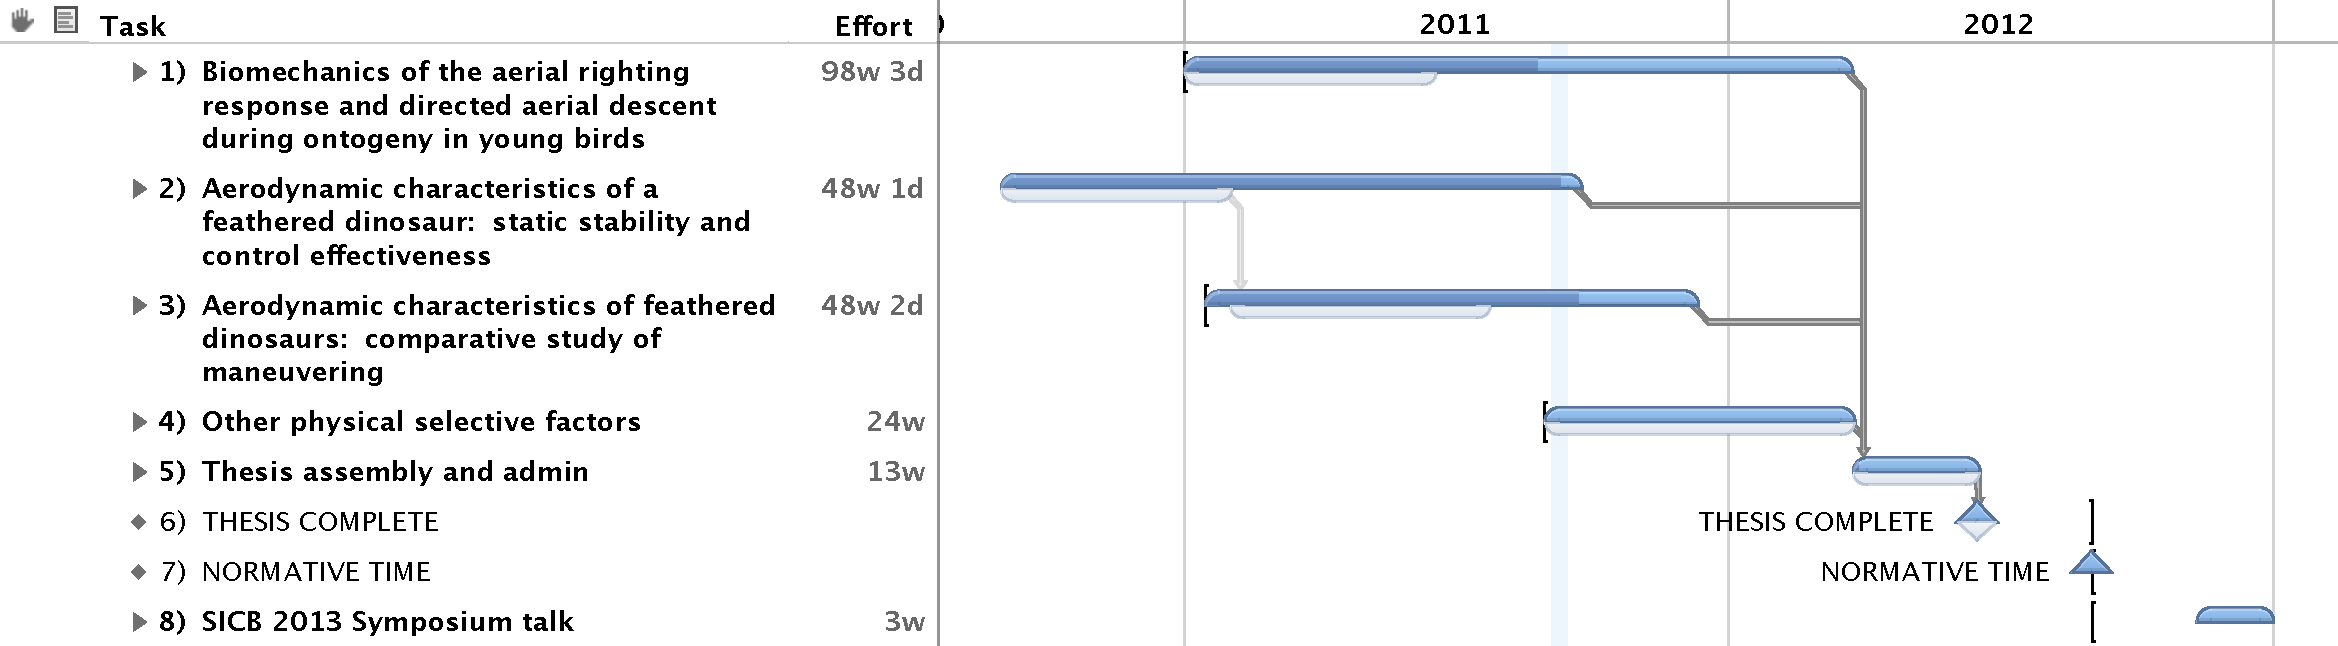
\includegraphics[width=9in]{figures/thesis-schedule-gantt.pdf}
\end{sidewaysfigure}


\appendix
\rcsid{$Id$}
\rcsid{$Header$}
\rcskwsave{$Author$}
\rcskwsave{$Date$} 
\rcskwsave{$Revision$}

\chapter{\emph{Alectoris chukar} Animal Use Protocol}
\label{app:AUP}
\index{Chukar}
\index{Alectoris chukar@\textit{Alectoris chukar}}
\index{Animal Use Protocol|(}
The following are excerpts from UC Berkeley Animal Use Protocol R282, revision 1 for the use of Chukars (\emph{Alectoris chukar}) in studies of directed aerial descent and righting.

\section{Research goals}
\index{Animal Use Protocol!goals}
Existing paleobiological scenarios for the origin of flapping flight in bats, birds, and pterosaurs strongly implicate transition from a gliding and maneuvering form, but the biomechanical and aerodynamic correlates of this transition are unclear. To examine biomechanical constraints relevant to such a transition, recent and past work includes studies of falling geckos \citep{Jusufi:2008}, gliding frogs \citep{Emerson:1990, McCay:2001}, extinct feathered dinosaurs \citep{Xing:2003}, and flying squirrels.  Other parallel work in invertebrate taxa, such as gliding ants \citep{Yanoviak:2005} and gliding stick insects also strongly implicate transition from a gliding and maneuvering form.

An alternate scenario for the origin of flapping flight in vertebrates involves the use of wings to assist running and traction up steep terrain \citetext{wing-assisted incline running, \citealp{Dial:2003, Bundle:2003, Dial:2008}}.  Studies in support of this alternative scenario have observed that hatchling birds utilize flapping movements when running up inclines \citep{Dial:2008}.   However, these studies ignore use of the wings during other aerial-related behaviors, for example, use of the wings when descending vertically.  Using the same species and general experimental setup, we plan to address this gap by determining limb and body kinematics, both symmetric and asymmetric, that contribute to aerial righting and directed aerial descent maneuvers, and that may have historically led to bilateral limb flapping in birds.  Wind tunnel studies of static and flapping models and computer simulations based on aerodynamics and inertial mechanics will complement these kinematic studies.


\section{Justification for animal use}
\index{Animal Use Protocol!justification for animal use}
\subsection{Rationale for use of animals}
Flying and gliding animals are paradigmatic examples of the generation and control of unsteady aerodynamic forces, and exhibit both neuromuscular regulation and multimodal sensory integration that far surpass current technological capacities.  To understand both generation and control of these aerodynamic phenomena, it is necessary to study living animals as they naturally locomote in the air.

\subsection{Rationale for choice of species and numbers}
Chukar Partridges are a model system for wing-assisted inclined running; as this work examines a gap in WAIR theory and seeks to extend it, they are a logical choice to start with as the data obtained will be directly comparable to previous studies \citep{Bundle:2003, Dial:2003, Dial:2008}.  Chukars are widely available through the poultry trade \citep{Heinrichs:2009, OToole:2003, Willis:2009}.  The number of study birds is based on our lab�s previous work in similar kinematic studies and should provide sufficient replicate measurements. \index{Animal Use Protocol!species rationale}\index{Animal Use Protocol!number rationale}


\section{Description of laboratory research}
\index{Animal Use Protocol!research description}
With Chukar Partridges, we seek to determine 1) the presence or absence of an aerial righting reflex over ontogeny; 2) the presence or absence of directed aerial descent ability over ontogeny; 3) three-dimensional trajectories and limb and tail usage during such maneuvers; and 4) the impact of a limited set of non-invasive manipulations (attachment/augmentation of feathers, especially pelvic wing feathers \citep{Lippincott:1920, Xing:2003, Thomas:1997, Evans:1992, Evans:1994} and augmentation of tail inertia \citep{Jusufi:2008}.  

All experiments will involve filming with video cameras illuminated with \SI{500}{\watt} lights.  Each filming event lasts up to thirty seconds.  Birds may be filmed on a daily basis for periods of three hours  During all experiments, animals will be observed for signs of weakness and will be removed from the study if such signs are evident.  Animals showing signs of reluctance will be given time to habituate to experimental setups.  Animals may be non-destructively marked by either attachment of adhesive-backed \SI{3}{\milli\meter} reflectors  or use of Wite-out and black marker, both typical in other studies of bird locomotion \citep{Dial:2008, Hedrick:2007, Daley:2007, Essner:2002, Wischusen:1989}.  During marking, animals will be restrained by hand.


\subsection{Presence or absence of aerial righting reflexes over ontogeny}
Chicks will be placed on a platform such as a ladder and allowed to take off freely, or dropped at a random orientation by tipping out of a cup.  Their vertical orientation will be observed during descent using high-speed video recording of kinematics.  Gentle vibration may be applied to the cup to induce takeoff.  The experimental setup will provide for a soft landing area, such as a loosely spanned, soft and eleastic cloth or foam.  The methods here will be identical to those we have used to study aerial righting and directed aerial descent in rain forest canopy ants, stick insects, and also in geckos \citep{Jusufi:2008}.\index{Animal Use Protocol!kinematics}

All chukar experiments will be conducted using a ladder, ramp, or scaffold structure within a \SI{5 x 3}{\meter} full-ceiling-height animal enclosure with fabric or netting walls in Haas 97/99.  For runs in which voluntary bird behavior is recorded, filming will be conducted up to daily for up to three hours per day.  For runs in which birds are gently stimulated, \SI{5}{\minute} rest periods will be provided between glides and a \SI{30}{\minute} rest every five glides, with an absolute maximum of 15 glides per animal per day. \index{Animal Use Protocol! drop tests} 

\subsection{Presence or absence of directed aerial descent ability over ontogeny}
Using methods similar to \citep{Dial:2008}, chicks will be allowed to run up an incline and jump off it freely; or will be placed at the top of an obstacle and gently stimulated to descend from it into a soft landing area. Filming of the descent with multiple high-speed video cameras will assess if trajectories show evidence of turns or if they are random or confined to a single plane \citep{Essner:2002, Socha:2002}.  Most runs will film the free, volitional behavior of chicks as they explore the experimental setup.  

To provide additional testing of the extent of directed aerial descent abilities, the target landing zone may be displaced over small distances after the chick jumps, as has been done in what was done in previous studies of flying squirrels \citep{Wischusen:1990}.

\subsection{Three-dimensional trajectories and limb and tail usage during such maneuvers}
Part of this experiment will be conducted concurrently with experiments 1 and 2, which already film the animals using multiple high-speed video cameras that are sufficient to obtain three-dimensional trajectories and appendage use during maneuvers.  

To obtain additional information on aerodynamic use of appendages , chicks may be placed in the working section of a vertical wind tunnel  to simulate conditions of free fall \citep{McCay:2001, Jusufi:2008}. Equilibrium gliding at terminal falling velocity is reached when the aerodynamic drag and lift forces balance the force of gravity. A small animal like a Chukar Partridge will attain terminal velocity at a ventral airflow of less than \SI{6}{\meter\per\second}, depending on individual mass and surface area.  Chicks will not be exposed to air speeds exceeding the equivalent of individual terminal velocity. To prevent chicks from maneuvering sideways out of the test section and to enable high-speed video filming, transparent acrylic sidewalls will be mounted around the opening of the wind tunnel. A safety net will be installed in the test section to prevent animals from contacting the expansion chamber of the wind tunnel.\index{Animal Use Protocol! use of wind tunnel}


\subsection{Relative effects of inertia and aerodynamic forces in maneuvers}
 To examine the role of inertia, small weights no more than \SI{10}{\percent} of body weight will be attached to the chicks using veterinary wrap, similar to methods used in \citep{Daley:2007}.  Inertia will be increased by addition of a ``prosthetic tail'' made from a lightweight shaft (e.g. music wire, wood, plastic or cut turkey feathers) with a small weight held onto to the chick�s natural tail using veterinary wrap.  For control purposes, an equivalent amount of weight may be added at the hips, near the center of mass, or on a leg or wing \citetext{as in \citealp{Daley:2007}}. Weights will be removed at the end of each session. index{Animal Use Protocol!inertial augmentation}
 
To examine the role of aerodynamic forces, we will observe aerial behaviors over ontogeny as the bird�s natural feathers develop.  In addition, we may clip the primary feathers and retrices, augment the primary feathers or retrices by gluing of additional feather extensions \citetext{\citealp{Evans:1994}, approved UCB Animal Use Protocol R282}, or augment feathers by gluing flight feathers at the position of other, non-flight feathers such as the pelvic ``wing'' plumage \citep{Lippincott:1920}.
 
Feather extensions will be conducted using the method of \citet{Evans:1994}.  Feathers will be cut near the base and new feathers glued on to vary length from between \SIrange{5}{10}{\percent} of the original length.  Feather extensions will be glued using a combination of pins and cyanoacrylate superglue.  Attached feathers will have been frozen several months to kill any parasites that may have been present. 
During these manipulations, chicks will be restrained by hand.  No anesthetization is necessary because the manipulations involve no living tissue; no living tissue is manipulated other than whole-body restraint for no more than \SI{10}{\minute} during these procedures.  Feathers are attached carefully so that they retain aerodynamic function; this method has been used extensively for other avian taxa \citep{Evans:1994, Evans:1992, Thomas:1997} and these authors report that manipulated birds folded their tails naturally and did not pick at or seem to unduly notice the manipulated feathers.  Maneuverability and aerodynamic performance of individuals with manipulations will be assessed using the methods described above.  Upon completion of manipulation experiments, manipulated feathers will be plucked to induce their replacement.  Birds that pick at extensions will have the extensions checked and adjusted as practicable and will be given time to acclimate, but extensive picking or grooming of the extensions may invalidate the experiment and such birds will be removed from study. \index{Animal Use Protocol!feather extensions}

\section{Method of euthanasia and disposition of specimens}
\index{Animal Use Protocol!euthanasia}
Euthanasia, if needed for Chukar Partridges at study's completion: overdose of isoflurane or carbon dioxide inhalation followed by bilateral thoracotomy.

\section{Proposed animal housing}
Chukar Partridges will be maintained within the Animal Behavior Research Suites on the fifth floor of VLSB.  Chukar Partridge chicks will be maintained within the Animal Behavior Research Suites on the fifth floor of VLSB.  Birds will be kept on brooder bedding litter (wood shavings, sawdust, compressed wood pellets, or other suitable material) changed bi-weekly or as necessary \citep{Heinrichs:2009, Willis:2009}.  Lamps will be provided to maintain a warm temperature as necessary \citep{Heinrichs:2009, Willis:2009}.  Birds will be kept in an enclosure with approximately 25 chicks to a \num{4 x 3} foot area \citep{Heinrichs:2009, Willis:2009}.  We will keep an individual Chukar Partridge for up to eight weeks, to allow completion study up to the point of being fully feathered and slightly beyond.  Most work will be completed at approximately four weeks.  Batches of chicks will not be mixed and additional space will be provided as birds age beyond four weeks (approximately \num{2} square feet per bird) \citep{Heinrichs:2009, Willis:2009}. \index{Animal Use Protocol!housing}

Chukar Partridge will be fed typical chick starter rations (\SI{20}{\percent} protein) in suitably designed feeding containers \citep{Heinrichs:2009, Willis:2009}.  OLAC personnel will feed the birds daily following standard UCB arrangements.  Diet will occasionally be supplemented with grit, vegetable material, or insect larvae \citep{Heinrichs:2009, Willis:2009}.  Water will be available at all times in suitably designed watering containers no more than a few inches deep \citep{Heinrichs:2009, Willis:2009}. \index{Animal Use Protocol!feeding}

When Chukar Partridges are returned to fifth floor housing after flight experiments, they will be monitored one hour after return and again the following morning to ensure normal behavior.  We typically check in on all of our animals one to two times daily independent of the occurrence of flight experiments.
	
\section{Breeding}
No breeding will be undertaken. \index{Animal Use Protocol!breeding}

\section{Capture and transportation of animals}
Chukar Partridges will be obtained as one-day-old chicks and shipped via standard shipping methods for poultry \citep{Heinrichs:2009, Willis:2009}.   For experiments, chicks will be transported between the Animal Behavior Research Suites on the fifth floor of VLSB and Haas 97/99 (a one minute walk) using a small animal carrier with litter and provision for ventilation.  No more than 12 chicks will be placed in one box (or less depending on size).  \index{Animal Use Protocol!transport of birds}

\section{Description of field research}
No field components are associated with studies of Chukar Partridges.\index{Animal Use Protocol!field research}

\index{Animal Use Protocol|)}



\pagestyle{plain}
\bibliography{references/thesis}
\printindex

\end{document}
